\documentclass[11pt,letterpaper]{article}

% Packages
\usepackage[utf8]{inputenc}
\usepackage[margin=1in]{geometry}
\usepackage{amsmath,amssymb,amsthm}
\usepackage{graphicx}
\usepackage{hyperref}
\usepackage{booktabs}
\usepackage{enumitem}
\usepackage{xcolor}
\usepackage{tikz}
\usetikzlibrary{arrows.meta,positioning,shapes}
\usepackage{algorithm}
\usepackage{algpseudocode}
\usepackage{subcaption}
\usepackage{natbib}
\usepackage{tcolorbox}

% Custom colors
\definecolor{claudecolor}{RGB}{204, 119, 34}
\definecolor{copilotcolor}{RGB}{36, 41, 46}
\definecolor{codexcolor}{RGB}{16, 163, 127}
\definecolor{julescolor}{RGB}{66, 133, 244}

% Title
\title{\textbf{Project Proposals: Network Analysis of AI Coding Tool Adoption on GitHub}}
\author{
    Alexander Quispe \\
    \textit{CS 145: Networks} \\
    \textit{California Institute of Technology}
}
\date{March 2026}

\begin{document}

\maketitle

\begin{abstract}
We present multiple project proposals analyzing the adoption and diffusion of AI coding assistants (Claude Code, GitHub Copilot, OpenAI Codex, and Google Jules) across the GitHub developer network. Using a novel dataset of 5+ million AI-assisted code contributions spanning 600,000+ repositories, we propose investigating cascade effects, social influence, and network dynamics in technology adoption. Each proposal includes motivation, methodology, network science foundations, and expected deliverables.
\end{abstract}

%==============================================================================
\section{Introduction and Dataset Overview}
%==============================================================================

The emergence of AI coding assistants represents one of the most significant technological shifts in software development history. Between February 2025 and January 2026, we collected comprehensive data on four major AI coding tools:

\begin{table}[h]
\centering
\caption{Dataset Summary: AI Coding Tool Usage on GitHub}
\label{tab:dataset}
\begin{tabular}{lrrrl}
\toprule
\textbf{Tool} & \textbf{Events} & \textbf{Repositories} & \textbf{Users (est.)} & \textbf{Detection Method} \\
\midrule
Claude Code & 281,058 & 438,979 & 50,000+ & Co-author trailers \\
GitHub Copilot & 1,082,564 & 246,957 & 200,000+ & Branch prefix \texttt{copilot/} \\
OpenAI Codex & 3,094,740 & 248,608 & 300,000+ & Branch prefix \texttt{codex/} \\
Google Jules & 622,121 & 70,116 & 20,000+ & Bot commits \\
\midrule
\textbf{Total} & \textbf{5,080,483} & \textbf{$\sim$600,000} & \textbf{500,000+} & --- \\
\bottomrule
\end{tabular}
\end{table}

This dataset enables unprecedented analysis of technology adoption dynamics in developer networks. Below we present six distinct project proposals, each offering a unique perspective on network effects in AI tool adoption.

%==============================================================================
\section{Project Proposal 1: Cascade Effects in AI Tool Adoption}
%==============================================================================

\subsection{The Idea}

\begin{tcolorbox}[colback=blue!5,colframe=blue!75!black,title=Core Question]
\textit{Does AI coding tool adoption spread through developer collaboration networks like an information cascade, and can we predict which developers will adopt based on their network position?}
\end{tcolorbox}

We propose modeling AI tool adoption as an \textbf{information cascade} through GitHub's developer collaboration network. When a developer sees their collaborators successfully using Claude Code or Copilot, they may be more likely to adopt the tool themselves. This creates cascade dynamics similar to those studied in viral marketing and social contagion.

\subsubsection{Network Construction}

We will construct a \textbf{developer collaboration network} $G = (V, E)$ where:
\begin{itemize}
    \item $V$ = set of developers (identified by GitHub username)
    \item $E$ = edges connecting developers who have contributed to the same repository
    \item Edge weights $w_{ij}$ = number of shared repositories between developers $i$ and $j$
\end{itemize}

\subsubsection{Cascade Model}

We adapt the \textbf{Independent Cascade Model} for AI tool adoption:

\begin{enumerate}
    \item At time $t=0$, a seed set $S_0$ of ``early adopters'' has adopted tool $T$
    \item At each time step $t$, newly adopted developers attempt to ``infect'' their neighbors
    \item Developer $j$ adopts from neighbor $i$ with probability:
    \[
    p_{ij} = \frac{w_{ij}}{\sum_k w_{ik}} \cdot \beta
    \]
    where $\beta$ is the base transmission rate (to be estimated)
\end{enumerate}

\subsubsection{Temporal Analysis}

Using our timestamped data, we can:
\begin{enumerate}
    \item Identify when each developer first adopted each tool
    \item Reconstruct the temporal sequence of adoptions
    \item Test whether adoption follows network structure
\end{enumerate}

\subsection{Motivation}

Understanding cascade dynamics has significant implications:

\begin{enumerate}
    \item \textbf{For AI companies}: Identify influential developers who can seed adoption
    \item \textbf{For researchers}: Understand how new technologies diffuse through professional networks
    \item \textbf{For organizations}: Predict which teams will adopt AI tools based on network position
\end{enumerate}

The network perspective goes beyond simple adoption curves by explaining \textit{why} certain developers adopt faster than others.

\subsection{Methodology}

\begin{algorithm}
\caption{Cascade Detection in AI Tool Adoption}
\begin{algorithmic}[1]
\State \textbf{Input:} Commits/PRs with timestamps, repository contributors
\State \textbf{Output:} Cascade trees, influence parameters
\State
\State Build collaboration graph $G$ from shared repository contributions
\State For each tool $T \in \{\text{Claude, Copilot, Codex, Jules}\}$:
\State \quad Extract adoption timestamps $\{(u_i, t_i)\}$ for each user
\State \quad Sort adoptions chronologically
\State \quad For each adoption $(u_j, t_j)$:
\State \quad\quad Find neighbors $N(u_j)$ who adopted before $t_j$
\State \quad\quad Assign most likely ``parent'' based on timing and edge weight
\State \quad Construct cascade tree
\State Estimate transmission parameters via maximum likelihood
\State Validate on held-out data (predict future adoptions)
\end{algorithmic}
\end{algorithm}

\subsection{Expected End Product}

\begin{enumerate}
    \item \textbf{Visualization}: Interactive cascade trees showing how adoption spread through the network
    \item \textbf{Model}: Calibrated Independent Cascade model with estimated parameters
    \item \textbf{Predictions}: Identify developers likely to adopt in the next 6 months
    \item \textbf{Paper}: Analysis comparing cascade dynamics across the four AI tools
\end{enumerate}

%==============================================================================
\section{Project Proposal 2: Social Influence vs. Homophily in Tool Selection}
%==============================================================================

\subsection{The Idea}

\begin{tcolorbox}[colback=green!5,colframe=green!75!black,title=Core Question]
\textit{Do developers adopt AI tools because their collaborators influenced them (social influence), or because similar developers independently make similar choices (homophily)?}
\end{tcolorbox}

This is the classic \textbf{identification problem} in network analysis: distinguishing causation from correlation. If two connected developers both use Claude Code, is it because:
\begin{itemize}
    \item \textbf{Influence}: One developer saw the other using it and was convinced to try it?
    \item \textbf{Homophily}: Both developers share characteristics (e.g., Python expertise) that independently predict Claude adoption?
    \item \textbf{Confounding}: Both developers work at the same company with an enterprise Claude license?
\end{itemize}

\subsection{Motivation}

This distinction has profound implications:
\begin{itemize}
    \item If \textbf{influence dominates}: Targeting influential developers can accelerate adoption
    \item If \textbf{homophily dominates}: Marketing should focus on developer characteristics, not network position
    \item Understanding the mechanism helps predict future technology adoption patterns
\end{itemize}

\subsection{Methodology}

We will apply several identification strategies:

\subsubsection{Temporal Analysis (Granger-style)}

If influence is real, adoption by neighbors at time $t-1$ should predict adoption at time $t$, even after controlling for individual characteristics:

\[
\text{Adopt}_{i,t} = \alpha + \beta \cdot \text{NeighborAdopt}_{i,t-1} + \gamma \cdot X_i + \epsilon_{i,t}
\]

where $X_i$ includes programming language, repository topics, geographic location, and account age.

\subsubsection{Matched Pair Analysis}

For each developer who adopted after a neighbor, find a ``matched'' developer with:
\begin{itemize}
    \item Same programming language profile
    \item Similar repository count
    \item Similar follower count
    \item BUT no neighbors who adopted
\end{itemize}

Compare adoption rates between matched and exposed developers.

\subsubsection{Network Randomization Tests}

Shuffle adoption times while preserving:
\begin{enumerate}
    \item Network structure
    \item Total number of adoptions per time period
    \item Individual developer characteristics
\end{enumerate}

If observed temporal clustering exceeds shuffled networks, influence is present.

\subsection{Expected End Product}

\begin{enumerate}
    \item \textbf{Quantification}: Decompose adoption into influence vs. homophily components
    \item \textbf{Comparison}: Which tool shows strongest network effects? (Hypothesis: Claude Code, due to visible co-author attribution)
    \item \textbf{Recommendations}: Evidence-based strategies for technology diffusion
\end{enumerate}

%==============================================================================
\section{Project Proposal 3: Multi-Tool Adoption as a Multiplex Network}
%==============================================================================

\subsection{The Idea}

\begin{tcolorbox}[colback=orange!5,colframe=orange!75!black,title=Core Question]
\textit{How do developers navigate the ecosystem of competing AI tools, and does adoption of one tool predict adoption or rejection of others?}
\end{tcolorbox}

Rather than analyzing each tool in isolation, we model the entire AI coding ecosystem as a \textbf{multiplex network} with four layers:

\begin{figure}[h]
\centering
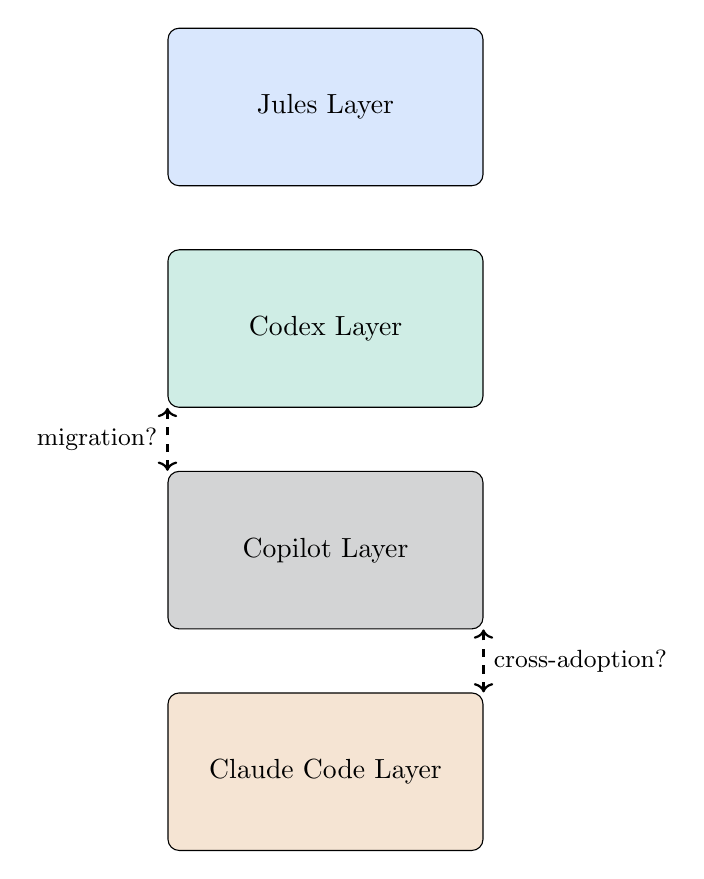
\begin{tikzpicture}[
    layer/.style={draw, minimum width=4cm, minimum height=2cm, rounded corners},
    node distance=0.8cm
]
    % Layers
    \node[layer, fill=claudecolor!20] (claude) {Claude Code Layer};
    \node[layer, fill=copilotcolor!20, above=of claude] (copilot) {Copilot Layer};
    \node[layer, fill=codexcolor!20, above=of copilot] (codex) {Codex Layer};
    \node[layer, fill=julescolor!20, above=of codex] (jules) {Jules Layer};

    % Cross-layer connections
    \draw[dashed, thick, <->] (claude.north east) -- (copilot.south east)
        node[midway, right] {\small cross-adoption?};
    \draw[dashed, thick, <->] (copilot.north west) -- (codex.south west)
        node[midway, left] {\small migration?};
\end{tikzpicture}
\caption{Multiplex network representation of AI tool ecosystem}
\end{figure}

\subsection{Research Questions}

\begin{enumerate}
    \item \textbf{Cross-adoption}: Do developers who use Claude Code also use Copilot?
    \item \textbf{Tool Migration}: Do developers switch from one tool to another over time?
    \item \textbf{Ecosystem Dynamics}: Is the market trending toward winner-take-all or coexistence?
    \item \textbf{Repository Heterogeneity}: Do repositories use multiple tools simultaneously?
\end{enumerate}

\subsection{Methodology}

\subsubsection{User Linking Across Tools}

Match developers across datasets using:
\begin{itemize}
    \item GitHub username (exact match)
    \item Repository co-occurrence (same repos with different tools)
\end{itemize}

\subsubsection{Multiplex Network Metrics}

\begin{itemize}
    \item \textbf{Layer correlation}: Are the same developers central in multiple layers?
    \item \textbf{Multiplexity}: How many layers does each developer participate in?
    \item \textbf{Inter-layer community detection}: Do communities align across tools?
\end{itemize}

\subsubsection{Transition Analysis}

Model tool switching as a Markov process:
\[
P(\text{Tool}_{t+1} = j \mid \text{Tool}_t = i) = \pi_{ij}
\]

Estimate transition matrix $\Pi$ from temporal adoption data.

\subsection{Expected End Product}

\begin{enumerate}
    \item \textbf{Market Map}: Visualization of tool ecosystem with adoption flows
    \item \textbf{Transition Matrix}: Quantified migration patterns between tools
    \item \textbf{Predictions}: Future market share based on current trends
    \item \textbf{Segmentation}: Developer archetypes (loyalists, explorers, pragmatists)
\end{enumerate}

%==============================================================================
\section{Project Proposal 4: Geographic Diffusion of AI Coding Tools}
%==============================================================================

\subsection{The Idea}

\begin{tcolorbox}[colback=red!5,colframe=red!75!black,title=Core Question]
\textit{How does AI coding tool adoption spread geographically, and are there regional leader-follower dynamics in technology adoption?}
\end{tcolorbox}

Using the \texttt{owner\_location} field in our repository metadata, we can analyze geographic patterns in AI tool adoption. This connects to literature on:
\begin{itemize}
    \item Spatial diffusion of innovation
    \item Technology adoption by country
    \item Time zone effects on open source collaboration
\end{itemize}

\subsection{Motivation}

Geographic analysis can reveal:
\begin{enumerate}
    \item Which regions are leading vs. lagging in AI tool adoption
    \item Whether adoption spreads through geographic proximity
    \item Cultural or regulatory factors affecting tool choice
    \item Opportunities for localized developer outreach
\end{enumerate}

\subsection{Methodology}

\subsubsection{Location Extraction and Geocoding}

\begin{enumerate}
    \item Parse \texttt{owner\_location} strings
    \item Geocode to country/region using NLP
    \item Handle ambiguous locations (``Bay Area'', ``Remote'')
\end{enumerate}

\subsubsection{Spatial Network Construction}

\begin{itemize}
    \item Nodes = countries or regions
    \item Edges = collaboration intensity (developers from different regions working on same repos)
    \item Edge weights = number of cross-region collaborations
\end{itemize}

\subsubsection{Spatial Diffusion Model}

Adapt epidemic models for spatial spread:
\[
\frac{dI_r}{dt} = \beta S_r \sum_{r'} w_{rr'} I_{r'} - \gamma I_r
\]

where $I_r$ is infected (adopted) proportion in region $r$, and $w_{rr'}$ is collaboration intensity between regions.

\subsection{Expected End Product}

\begin{enumerate}
    \item \textbf{World Map}: Animated visualization of tool adoption spreading geographically
    \item \textbf{Regional Analysis}: Adoption curves by country/continent
    \item \textbf{Leader-Follower}: Identify which regions set trends vs. follow
    \item \textbf{Comparison}: Do different tools have different geographic patterns?
\end{enumerate}

%==============================================================================
\section{Project Proposal 5: Influence Maximization for AI Tool Adoption}
%==============================================================================

\subsection{The Idea}

\begin{tcolorbox}[colback=purple!5,colframe=purple!75!black,title=Core Question]
\textit{Which developers should an AI company target to maximize adoption through network effects?}
\end{tcolorbox}

This is the classic \textbf{influence maximization problem}: given a budget to recruit $k$ ``seed'' developers, which $k$ developers will lead to maximum total adoption?

\subsection{Motivation}

For AI coding tool companies, this has direct business value:
\begin{itemize}
    \item Developer advocates and evangelists
    \item Open source sponsorship targets
    \item Conference speaker selection
    \item Beta program invitations
\end{itemize}

\subsection{Methodology}

\subsubsection{Network Construction}

Build collaboration network weighted by:
\begin{itemize}
    \item Number of shared repositories
    \item Recency of collaboration
    \item Size/importance of shared repositories (stars)
\end{itemize}

\subsubsection{Influence Maximization Algorithms}

Implement and compare:
\begin{enumerate}
    \item \textbf{Greedy algorithm}: Select node with maximum marginal influence gain
    \item \textbf{CELF/CELF++}: Cost-effective lazy forward selection
    \item \textbf{Degree heuristic}: Select highest-degree nodes
    \item \textbf{PageRank heuristic}: Select highest PageRank nodes
\end{enumerate}

\subsubsection{Validation}

Using historical data:
\begin{enumerate}
    \item Identify actual early adopters (first 10\% of adoptions)
    \item Compare to algorithm-selected seeds
    \item Measure downstream adoption from each seed set
\end{enumerate}

\subsection{Expected End Product}

\begin{enumerate}
    \item \textbf{Ranked Lists}: Top 100 influential developers for each tool
    \item \textbf{Algorithm Comparison}: Which approach works best for this domain?
    \item \textbf{ROI Analysis}: Expected adoption multiplier from seed selection
    \item \textbf{Tool}: Reusable influence maximization implementation
\end{enumerate}

%==============================================================================
\section{Project Proposal 6: Community Detection and Tool Ecosystem Clustering}
%==============================================================================

\subsection{The Idea}

\begin{tcolorbox}[colback=yellow!5,colframe=yellow!75!black,title=Core Question]
\textit{Do distinct communities form around different AI tools, and what characterizes these communities?}
\end{tcolorbox}

We hypothesize that developer communities may cluster by AI tool preference, programming language, or application domain. Understanding these communities helps predict adoption patterns.

\subsection{Methodology}

\subsubsection{Bipartite Network Analysis}

The natural structure is bipartite:
\begin{itemize}
    \item $U$ = set of developers
    \item $V$ = set of repositories
    \item Edges = contributions
\end{itemize}

We can project this to:
\begin{itemize}
    \item \textbf{Developer network}: Connect developers who share repositories
    \item \textbf{Repository network}: Connect repositories that share contributors
\end{itemize}

\subsubsection{Community Detection}

Apply multiple algorithms:
\begin{enumerate}
    \item \textbf{Louvain}: Modularity optimization
    \item \textbf{Infomap}: Information flow-based
    \item \textbf{Label Propagation}: Scalable for large networks
    \item \textbf{Spectral Clustering}: Eigenvector-based
\end{enumerate}

\subsubsection{Community Characterization}

For each detected community, compute:
\begin{itemize}
    \item Dominant programming language
    \item Common repository topics
    \item Geographic concentration
    \item AI tool preference distribution
\end{itemize}

\subsection{Expected End Product}

\begin{enumerate}
    \item \textbf{Community Map}: Visualization of developer communities colored by tool preference
    \item \textbf{Profiles}: Characterization of each major community
    \item \textbf{Prediction}: Community membership as predictor of tool adoption
    \item \textbf{Comparison}: How do communities differ across tools?
\end{enumerate}

%==============================================================================
\section{Summary: Recommended Project Selection}
%==============================================================================

\begin{table}[h]
\centering
\caption{Project Comparison Matrix}
\label{tab:comparison}
\begin{tabular}{lcccc}
\toprule
\textbf{Project} & \textbf{Difficulty} & \textbf{Novelty} & \textbf{Impact} & \textbf{Feasibility} \\
\midrule
1. Cascade Effects & Medium & High & High & High \\
2. Influence vs. Homophily & High & Very High & Very High & Medium \\
3. Multiplex Network & Medium & High & Medium & High \\
4. Geographic Diffusion & Medium & Medium & Medium & High \\
5. Influence Maximization & Medium & Medium & High & High \\
6. Community Detection & Low-Medium & Medium & Medium & Very High \\
\bottomrule
\end{tabular}
\end{table}

\subsection{Our Recommended Selection}

For a networks course project, we recommend:

\begin{enumerate}
    \item \textbf{Primary Project}: \textbf{Cascade Effects in AI Tool Adoption} (Proposal 1)
    \begin{itemize}
        \item Strong connection to course material (information cascades)
        \item Novel application domain (AI coding tools)
        \item Rich temporal data enables rigorous analysis
        \item Produces compelling visualizations
    \end{itemize}

    \item \textbf{Secondary Project}: \textbf{Social Influence vs. Homophily} (Proposal 2)
    \begin{itemize}
        \item Addresses fundamental question in network science
        \item Methodologically sophisticated
        \item High potential for surprising findings
        \item Publishable research potential
    \end{itemize}
\end{enumerate}

%==============================================================================
\section{Technical Appendix: Data Processing Pipeline}
%==============================================================================

\subsection{Network Construction Code Outline}

\begin{verbatim}
# Build developer collaboration network
import pandas as pd
import networkx as nx

# Load commit data
commits = pd.read_parquet("claude_commits.parquet")

# Build repo -> developer mapping
repo_devs = commits.groupby("repo_nwo")["author_login"].apply(set)

# Build collaboration graph
G = nx.Graph()
for repo, devs in repo_devs.items():
    devs = list(devs)
    for i, d1 in enumerate(devs):
        for d2 in devs[i+1:]:
            if G.has_edge(d1, d2):
                G[d1][d2]["weight"] += 1
            else:
                G.add_edge(d1, d2, weight=1)
\end{verbatim}

\subsection{Cascade Detection Outline}

\begin{verbatim}
# Detect adoption cascades
def detect_cascades(G, adoptions):
    """
    adoptions: DataFrame with columns [user, timestamp]
    Returns: Dict mapping each adopter to their likely "parent"
    """
    cascades = {}
    sorted_adoptions = adoptions.sort_values("timestamp")
    adopted = set()

    for _, row in sorted_adoptions.iterrows():
        user = row["user"]
        # Find neighbors who adopted before this user
        neighbors = set(G.neighbors(user)) & adopted
        if neighbors:
            # Assign to most recent adopter among neighbors
            parent = max(neighbors,
                        key=lambda n: adoptions[adoptions.user==n].timestamp.max())
            cascades[user] = parent
        else:
            cascades[user] = None  # Seed node
        adopted.add(user)

    return cascades
\end{verbatim}

%==============================================================================
\section{References and Related Work}
%==============================================================================

Key papers to build upon:
\begin{enumerate}
    \item Kempe, D., Kleinberg, J., \& Tardos, E. (2003). Maximizing the spread of influence through a social network. \textit{KDD}.
    \item Aral, S., Muchnik, L., \& Sundararajan, A. (2009). Distinguishing influence-based contagion from homophily-driven diffusion. \textit{PNAS}.
    \item Centola, D. (2010). The spread of behavior in an online social network experiment. \textit{Science}.
    \item Bakshy, E., et al. (2012). The role of social networks in information diffusion. \textit{WWW}.
    \item Leskovec, J., et al. (2007). The dynamics of viral marketing. \textit{TWEB}.
\end{enumerate}

\end{document}
